\documentclass[11pt]{article}
\usepackage[margin=1in]{geometry}
\usepackage{graphicx}
\usepackage{booktabs}
\usepackage{tabularx}

\begin{document}

\section{Data Preprocessing and Missing-Value Handling}

Records with an invalid timestamp, a missing station identifier, a missing
rainfall value, or a negative rainfall value were removed. Zero rainfall was
retained because it represents a valid observation rather than missing data.

Each station is expected to provide 288 five-minute observations per day. A
station-day was retained when at least 95\% of these observations were
available. Its daily rainfall was divided by the observed coverage ratio to
make a small adjustment for the missing intervals. Days represented by fewer
than 30 valid stations were excluded from the Singapore-wide daily average.

Annual rainfall was estimated by multiplying the mean rainfall over valid
days by 365, or 366 in a leap year. This is reported as a coverage-adjusted
estimate because it assumes that missing days are similar to the observed
days. In the year-month heatmap, a cell was shown only when at least 15 valid
dates were available. The station map included only stations with at least
365 valid days. For the hourly analysis, only station-hours containing all 12
five-minute observations were retained.

\section{Task 1 Implementation}

Task 1 was implemented with PySpark in local mode, using four CPU threads and
4~GB of driver memory. The annual CSV files were read with a fixed schema and
combined into one Spark DataFrame. Spark transformations were then used to
clean the records and produce station-day, Singapore-wide daily, and
station-hour datasets. The annual, monthly, year-month, hourly, and station
summaries were calculated with Spark grouping operations. Only these small
summary tables were converted to pandas for plotting with Matplotlib and
Seaborn. Each plot was saved as a PNG file, and its underlying summary data was
also saved as a CSV file so that the reported values could be checked easily.

Table~\ref{tab:runtime-configuration} records the local machine and software
environment used to run Task 1. Package versions were read directly from the
\texttt{dsa5208proj2} Conda environment.

\begin{table}[htbp]
    \centering
    \caption{Local machine and software environment used for Task 1.}
    \label{tab:runtime-configuration}
    \small
    \begin{tabularx}{\textwidth}{@{}p{0.25\textwidth}p{0.34\textwidth}X@{}}
        \toprule
        Component & Configuration & Notes \\
        \midrule
        Operating system & Windows 11 Home, 64-bit (build 10.0.26200) & Chinese-language edition. \\
        Processor & Intel Core i7-12800HX & 16 physical cores and 24 logical processors. \\
        System memory & 15.7 GB RAM & Total visible memory reported by Windows. \\
        Graphics & NVIDIA GeForce RTX 4070 Laptop GPU; Intel UHD Graphics & Task 1 used CPU-based local Spark execution. \\
        Conda environment & \texttt{dsa5208proj2} & Managed with Conda 24.7.1. \\
        Python & CPython 3.10.22 & Environment interpreter. \\
        Java & Temurin OpenJDK 17.0.20.1 & Java runtime used by Spark. \\
        PySpark & 4.2.0 & \texttt{local[4]} mode with 4 GB driver memory. \\
        Data libraries & pandas 2.3.3; NumPy 2.2.6 & Used for small summary tables and array operations. \\
        Plotting libraries & Matplotlib 3.10.9; Seaborn 0.13.2 & Used to create the report figures. \\
        \bottomrule
    \end{tabularx}
\end{table}

\section{Task 1: Rainfall Patterns}

The following analysis uses the cleaned data described above. The figures
compare rainfall by year, month, hour, and monitoring station. Since station
coverage is not identical throughout the dataset, the values should be viewed
as useful summaries of the observed pattern rather than exact totals for the
whole of Singapore.

\subsection{Annual pattern}

Figure~\ref{fig:annual} shows that annual rainfall changed considerably from
2017 to 2024. The lowest estimate was in 2019, at about 1,727~mm, while the
highest was in 2022, at about 2,929~mm. Rainfall was also relatively high in
2021 and 2023. The 2024 estimate fell to about 2,700~mm, but it was still much
higher than the 2019 value. Overall, the plot does not show a simple increasing
or decreasing trend. Instead, wet and dry years occurred within the study
period.

The number above each bar gives the number of valid dates used. Most years had
more than 340 valid dates, but 2018 had only 266. Therefore, the 2018 estimate
is less reliable than the other annual estimates and should be interpreted
with more care.

\begin{figure}[htbp]
    \centering
    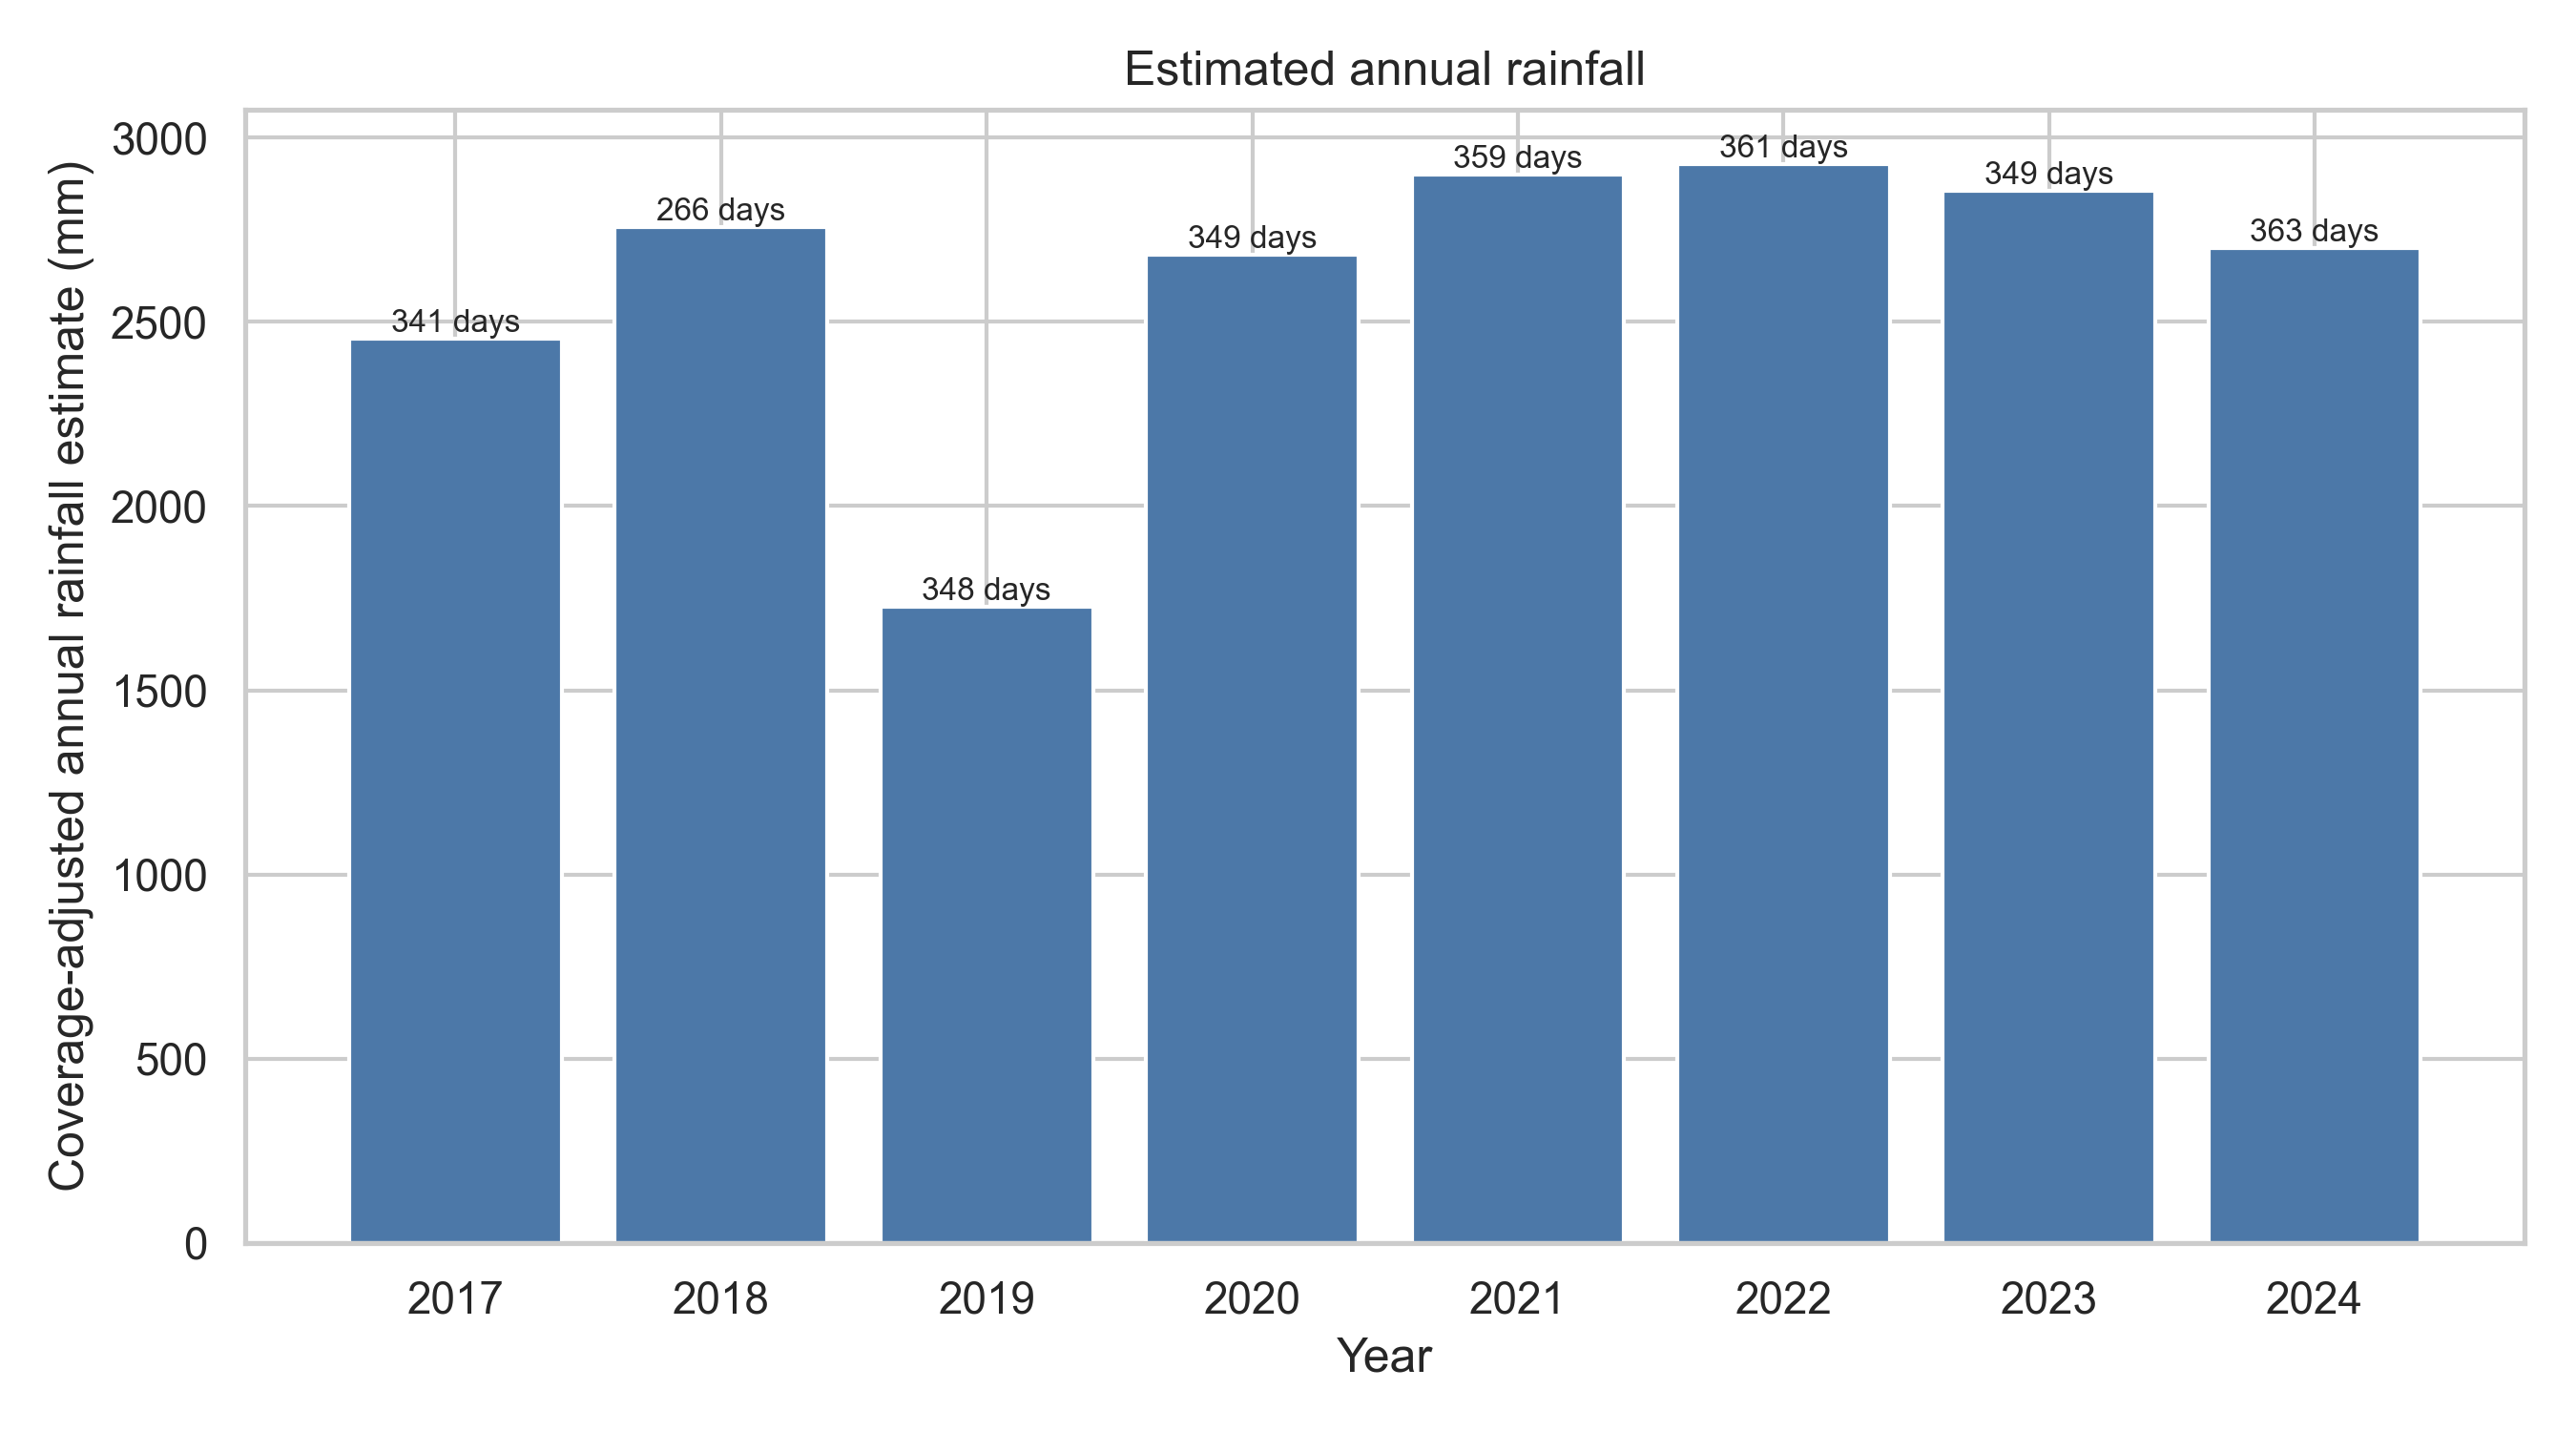
\includegraphics[width=0.88\textwidth]{figures/annual_rainfall.png}
    \caption{Coverage-adjusted annual rainfall estimates from 2017 to 2024.}
    \label{fig:annual}
\end{figure}

\subsection{Monthly pattern}

The average daily rainfall by calendar month is shown in
Figure~\ref{fig:monthly}. November was the wettest month, with an average of
10.56~mm per day. December, April, and June were also relatively wet, with
daily averages of about 8~mm or more. July and February were the driest months,
both at about 4.9~mm per day, while August was also relatively dry.

This result suggests that rainfall was generally stronger near the end of the
year, especially in November and December. However, the rise in April and June
shows that the pattern is not a simple division between one wet season and one
dry season. Rain can be high at several different times of the year.

\begin{figure}[htbp]
    \centering
    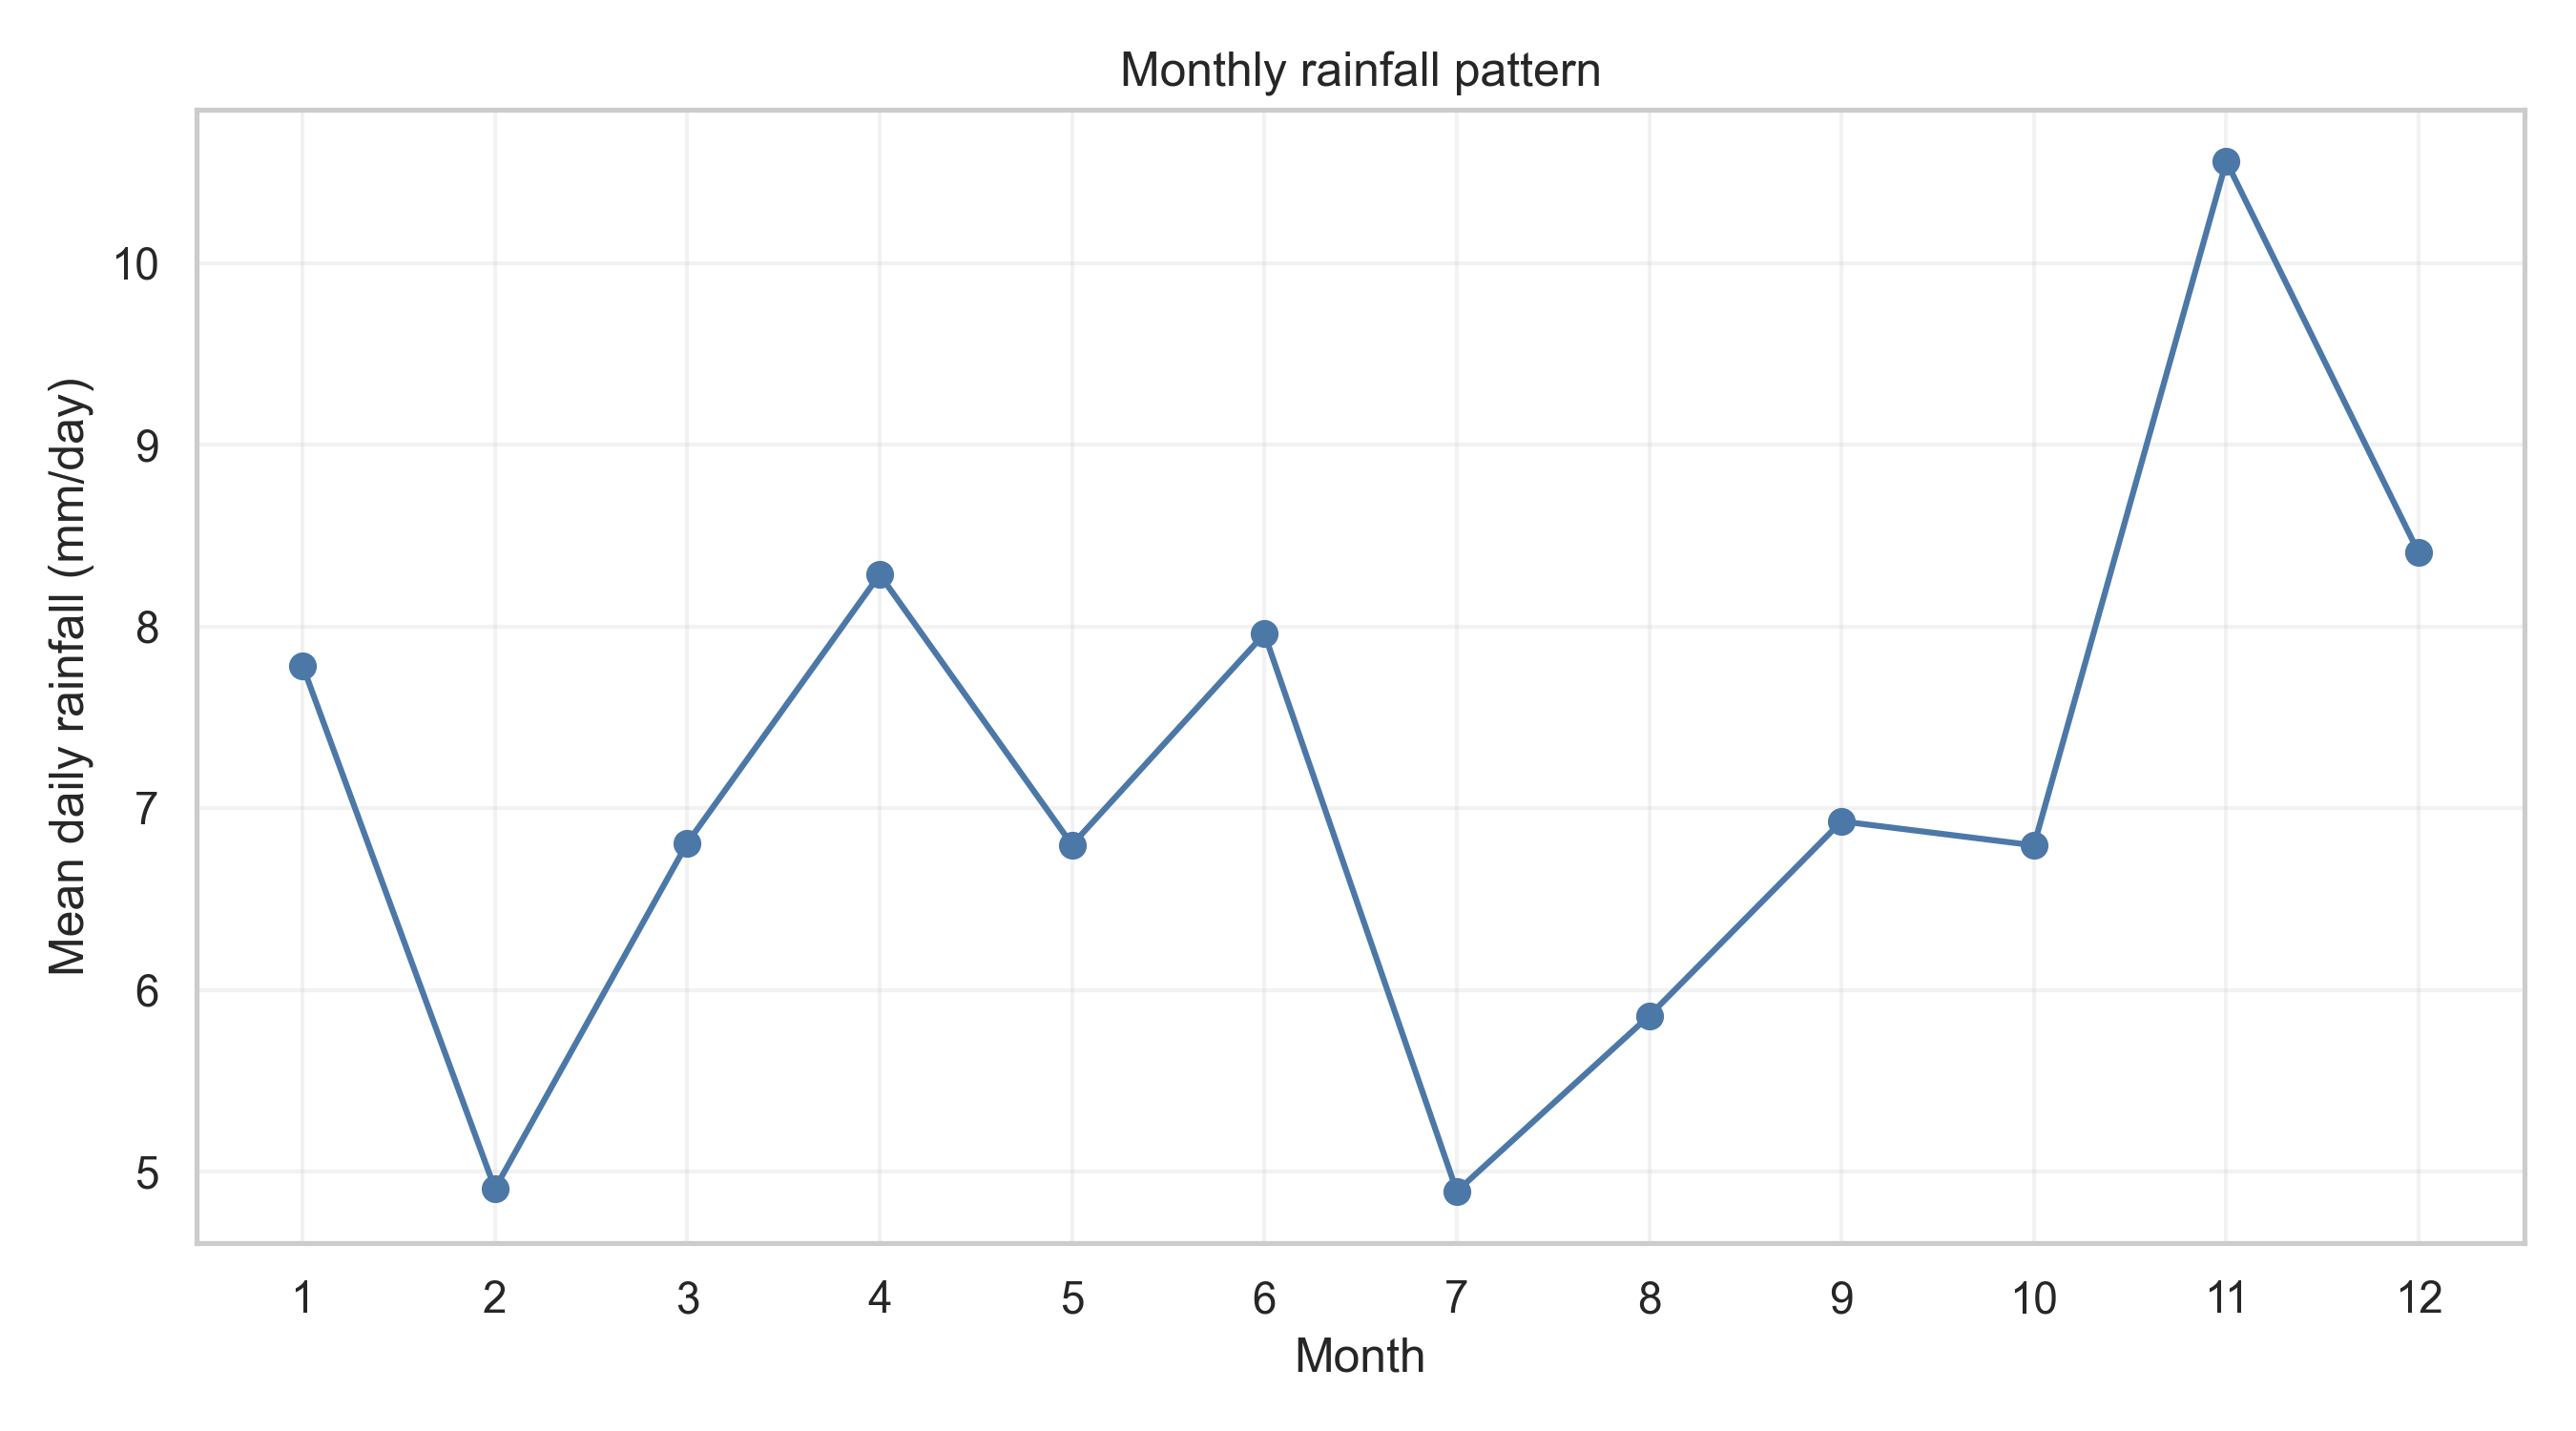
\includegraphics[width=0.88\textwidth]{figures/monthly_rainfall.png}
    \caption{Average daily rainfall for each calendar month, using data from
    2017--2024.}
    \label{fig:monthly}
\end{figure}

\subsection{Changes in monthly rainfall across years}

Figure~\ref{fig:heatmap} gives a more detailed view by separating every year
and month. The colours vary greatly across the heatmap, which means that the
same calendar month can behave quite differently in different years. For
example, August was very wet in 2021, at 13.21~mm per day, but August 2019 was
the driest displayed cell, at only 1.16~mm per day. Other very wet periods
included October 2022 (13.53~mm per day) and November 2024 (14.07~mm per day).

The heatmap therefore supports the annual and monthly results: there is a
general seasonal pattern, but it is not repeated in exactly the same way every
year. The blank cells in 2018 are not zero-rainfall months. They were left
blank because fewer than 15 valid dates were available, so there was not enough
data for a reasonable monthly comparison.

\begin{figure}[htbp]
    \centering
    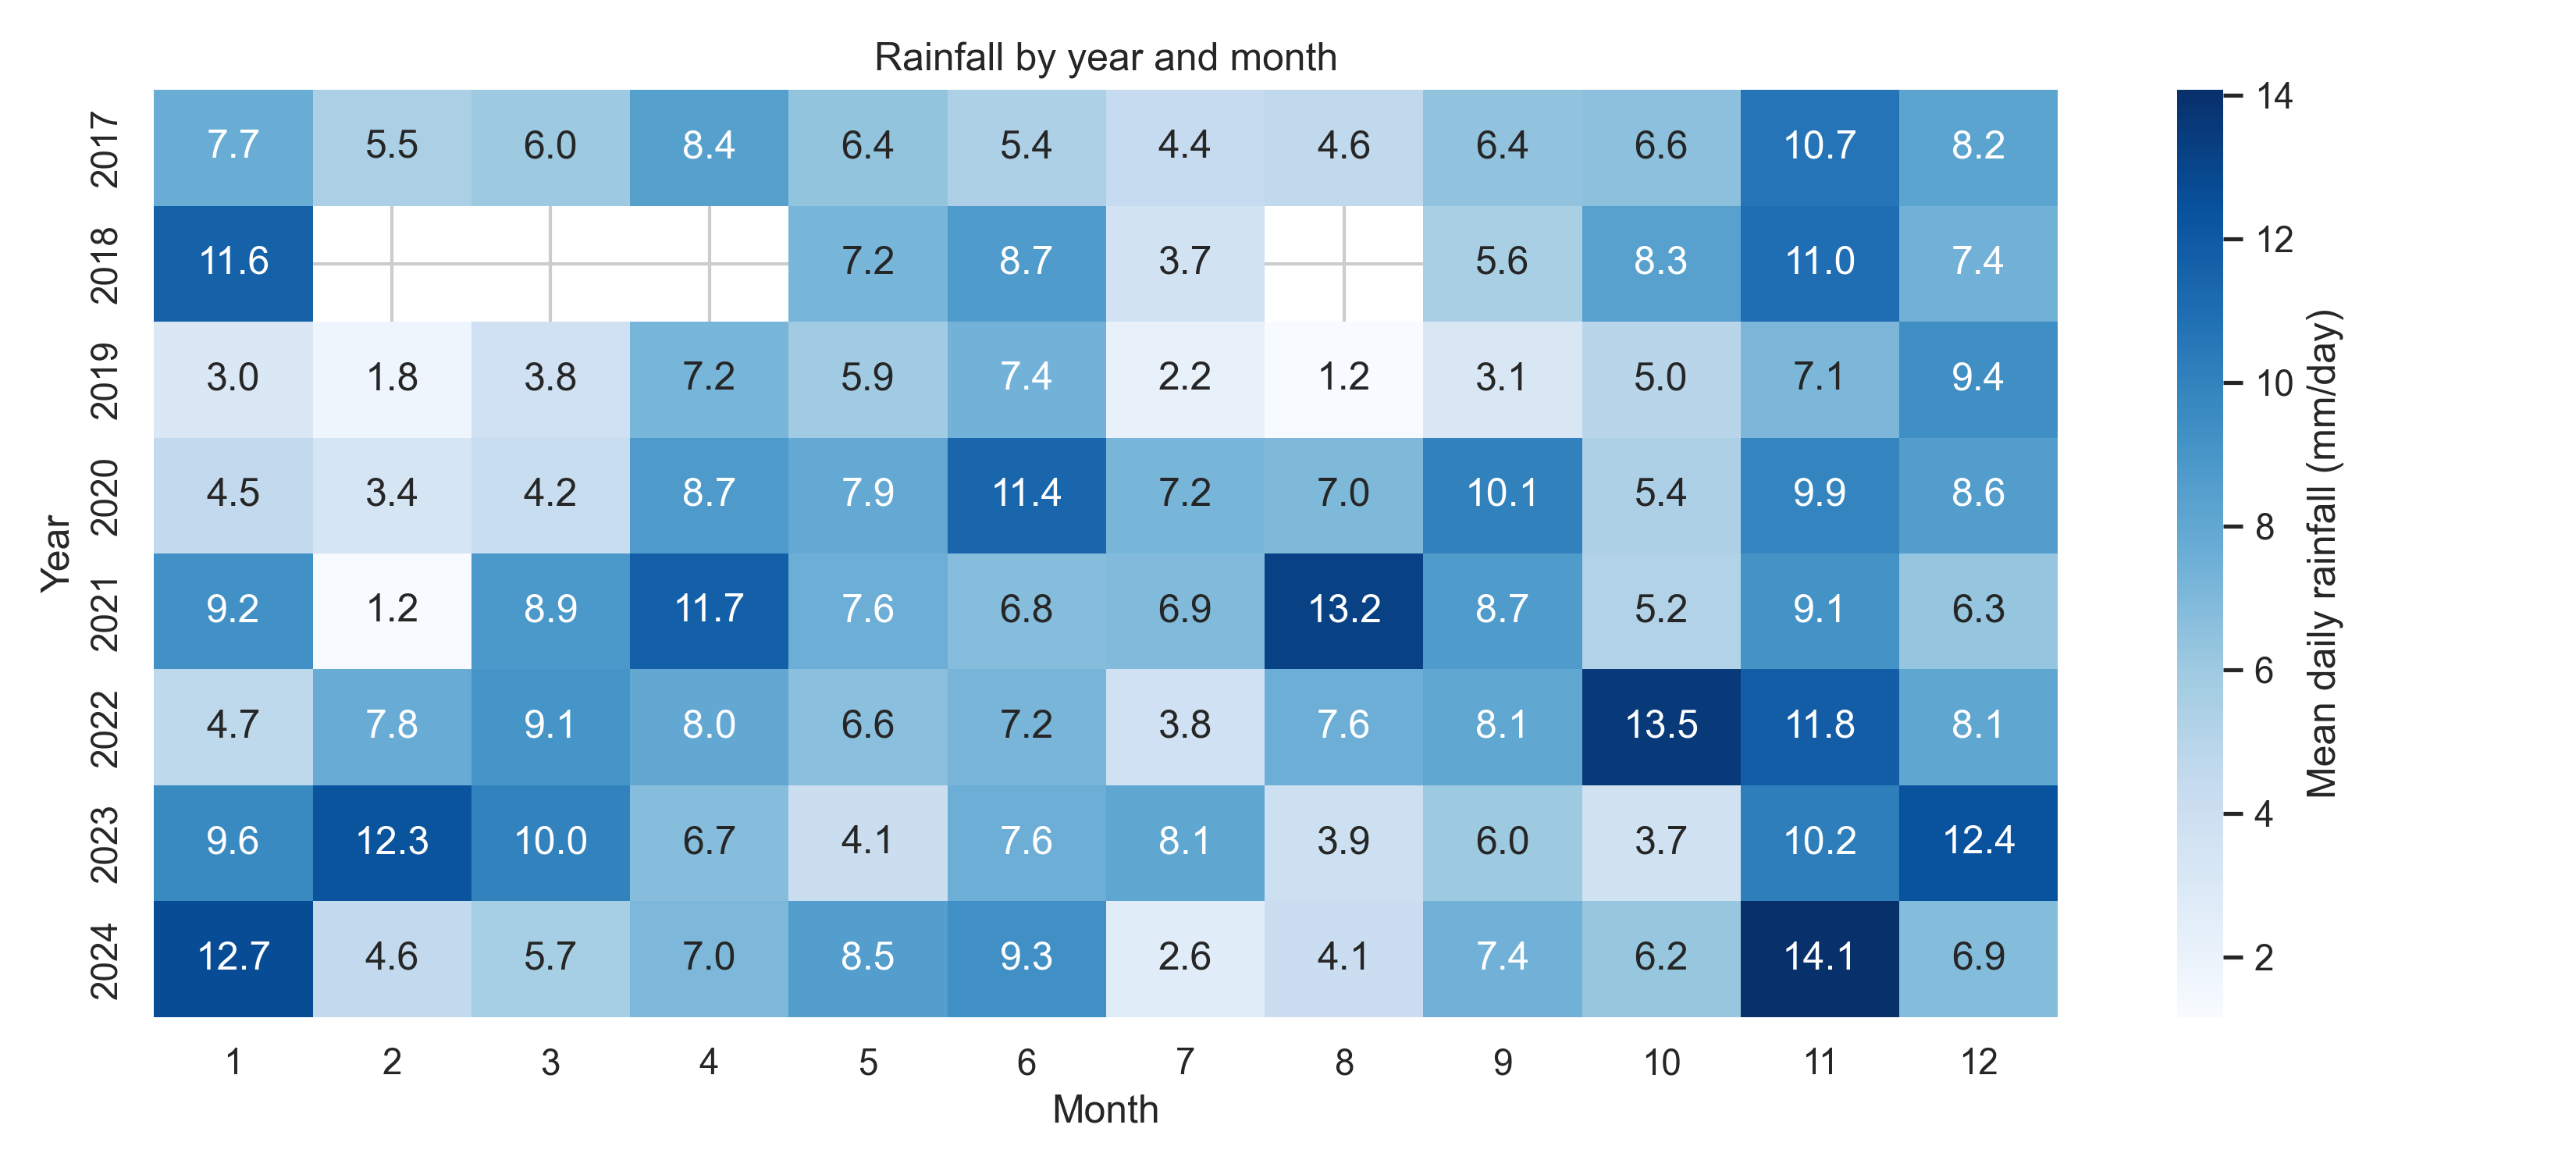
\includegraphics[width=0.95\textwidth]{figures/year_month_heatmap.png}
    \caption{Mean daily rainfall by year and month. Blank cells do not meet the
    minimum requirement of 15 valid dates.}
    \label{fig:heatmap}
\end{figure}

\subsection{Hourly pattern}

Figure~\ref{fig:hourly} shows a clear daily pattern. Rainfall was generally low
during the night and early morning, then increased from late morning and
reached its highest level in the afternoon. At 15:00, the mean hourly rainfall
was about 0.80~mm and the probability of a wet hour was about 15.8\%. Both
measures then decreased during the evening. The lowest mean hourly rainfall
was around 22:00, at about 0.09~mm.

The two lines have similar shapes, so the afternoon peak is seen in both the
amount of rainfall and the chance of observing rain. This makes time of day a
potentially useful feature for the rainfall prediction model in Task 2.

\begin{figure}[htbp]
    \centering
    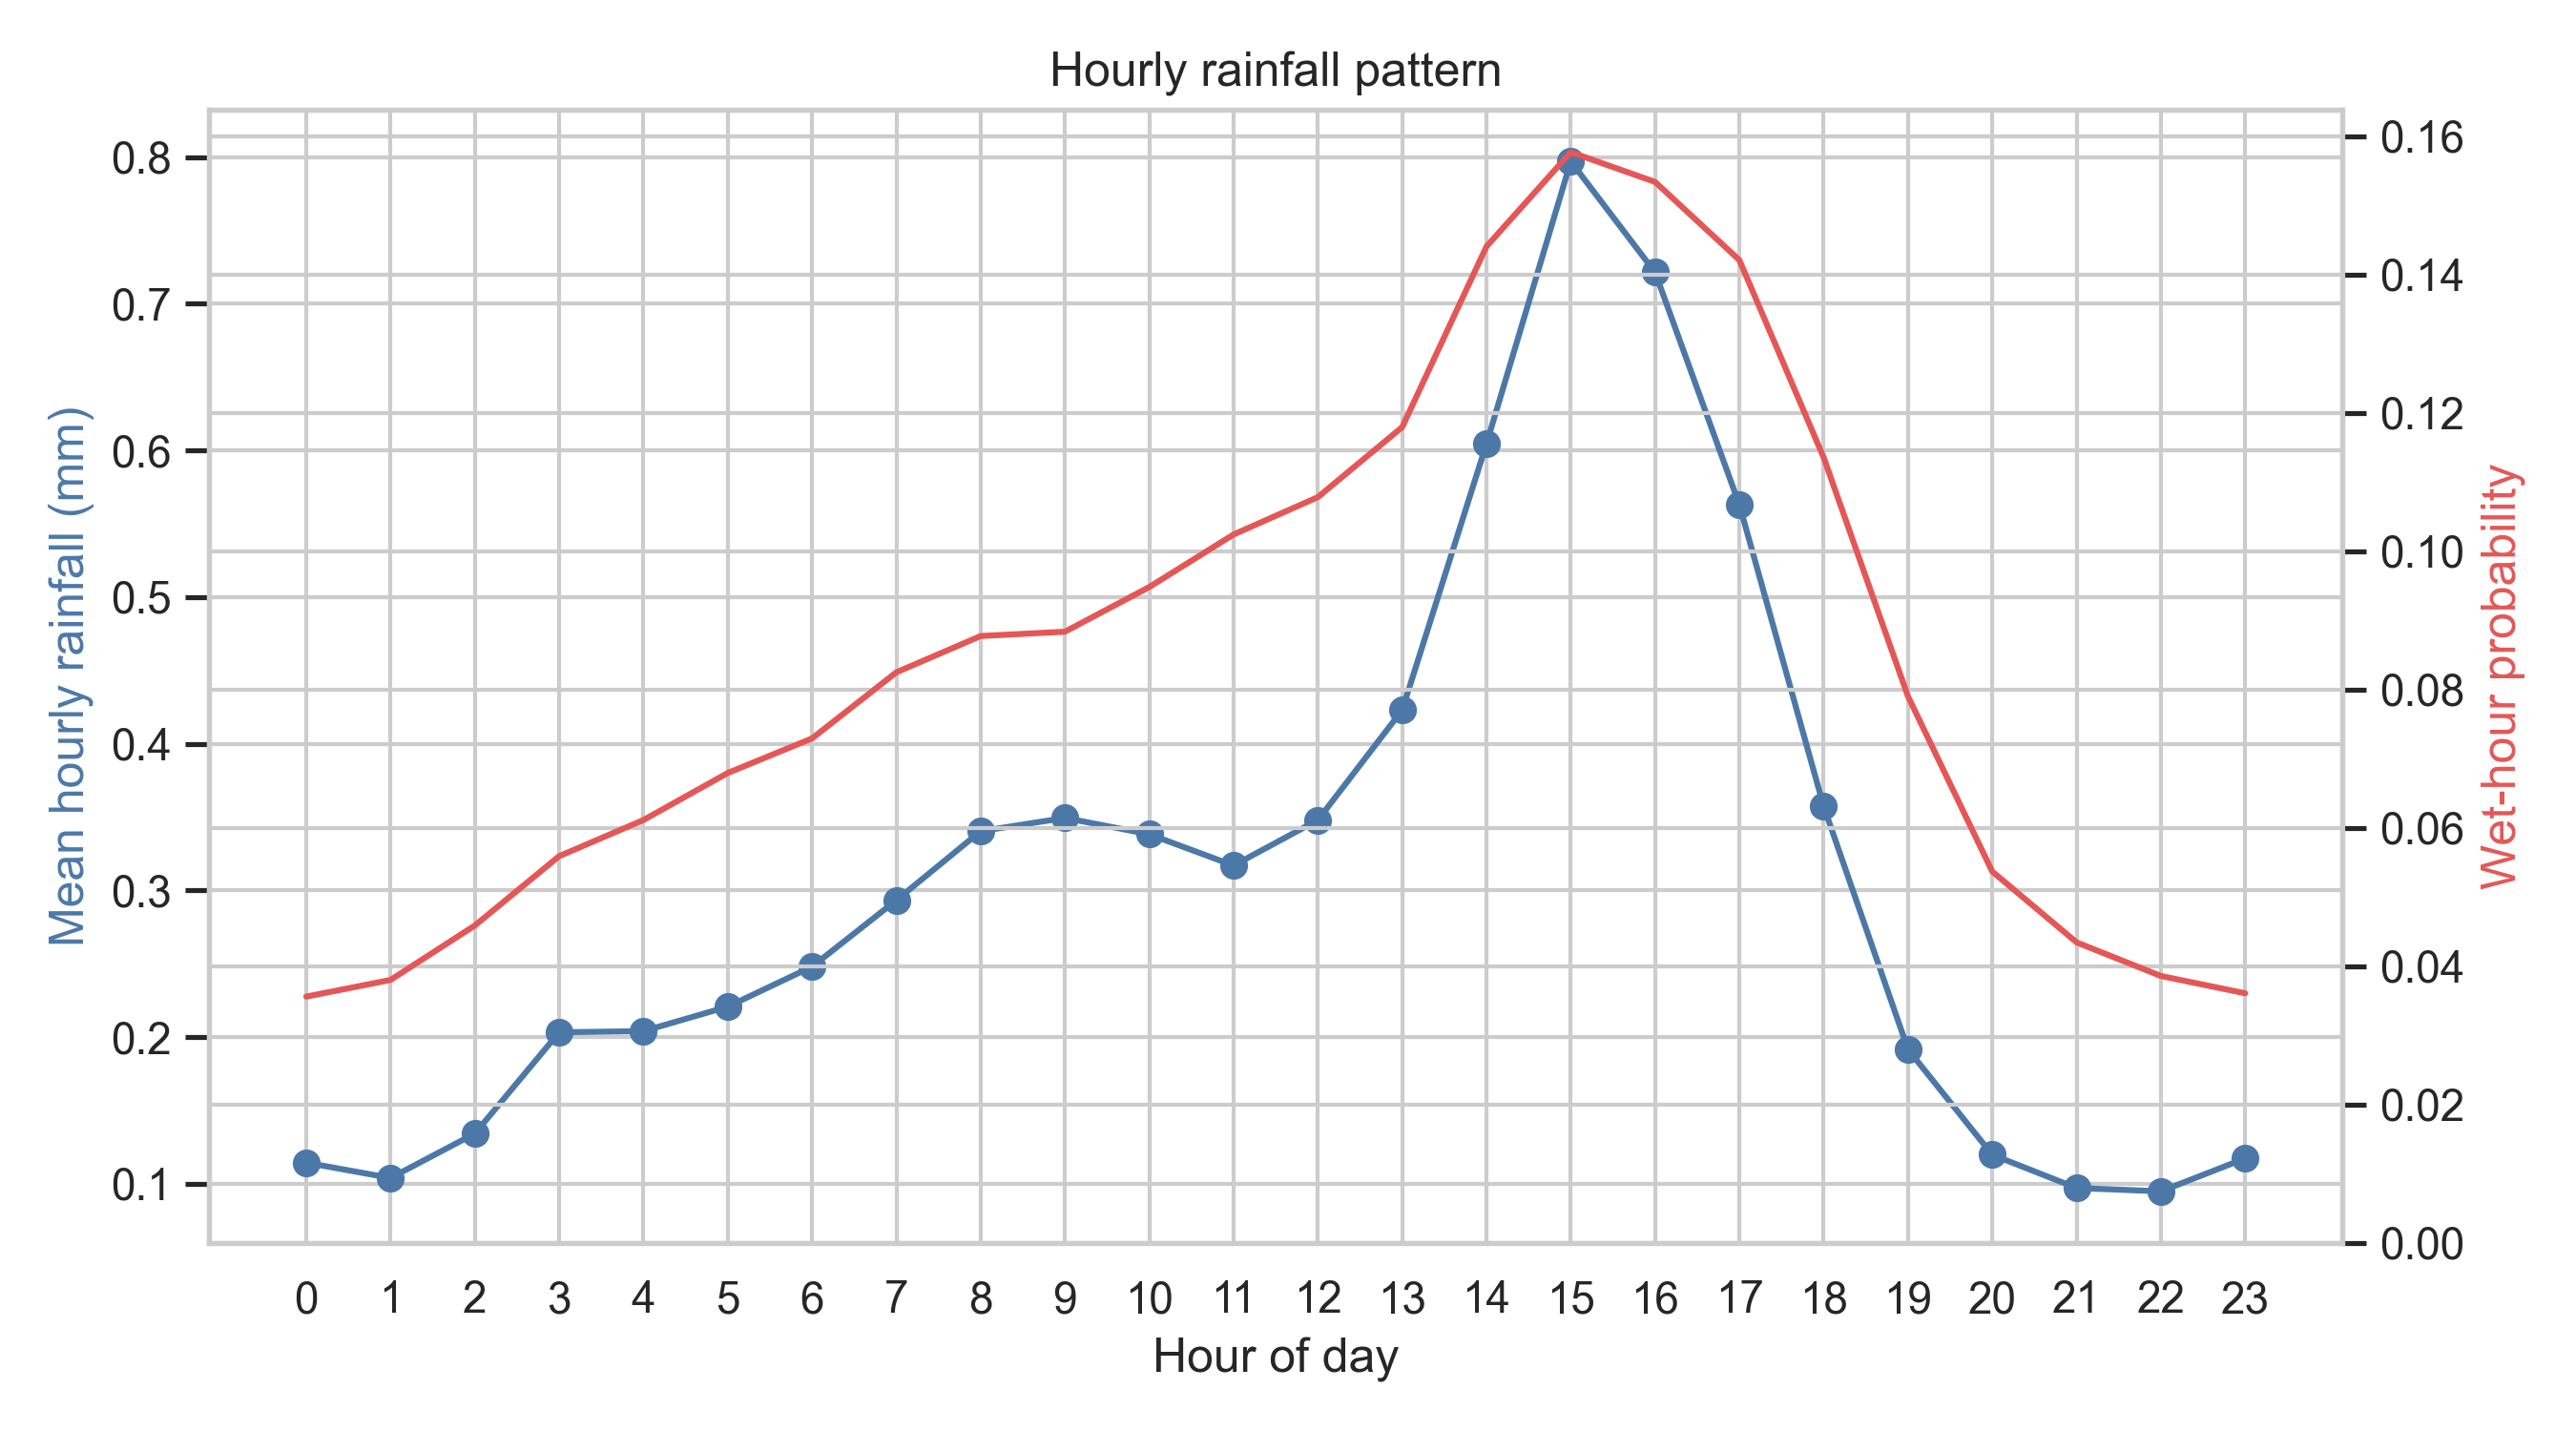
\includegraphics[width=0.9\textwidth]{figures/hourly_rainfall.png}
    \caption{Mean hourly rainfall and wet-hour probability by hour of day.}
    \label{fig:hourly}
\end{figure}

\subsection{Differences between monitoring stations}

The station map in Figure~\ref{fig:stations} contains 83 stations that met the
minimum data requirement. Their mean daily rainfall ranged from 4.84~mm to
9.76~mm. Station S228 had the highest value, followed by S203 and S202. Station
S208 had the lowest value, followed by S102 and S29.

Several stations in the west and central-west area have darker colours, while
some stations in the east and south have lighter colours. This suggests that
location is related to the amount of rainfall observed. However, the pattern
is not completely uniform, and station coverage also differs between places.
For this reason, the map is mainly used to show broad spatial differences, not
to claim that every western location is wetter than every eastern location.
Station identity or location may also be useful inputs for Task 2.

\begin{figure}[htbp]
    \centering
    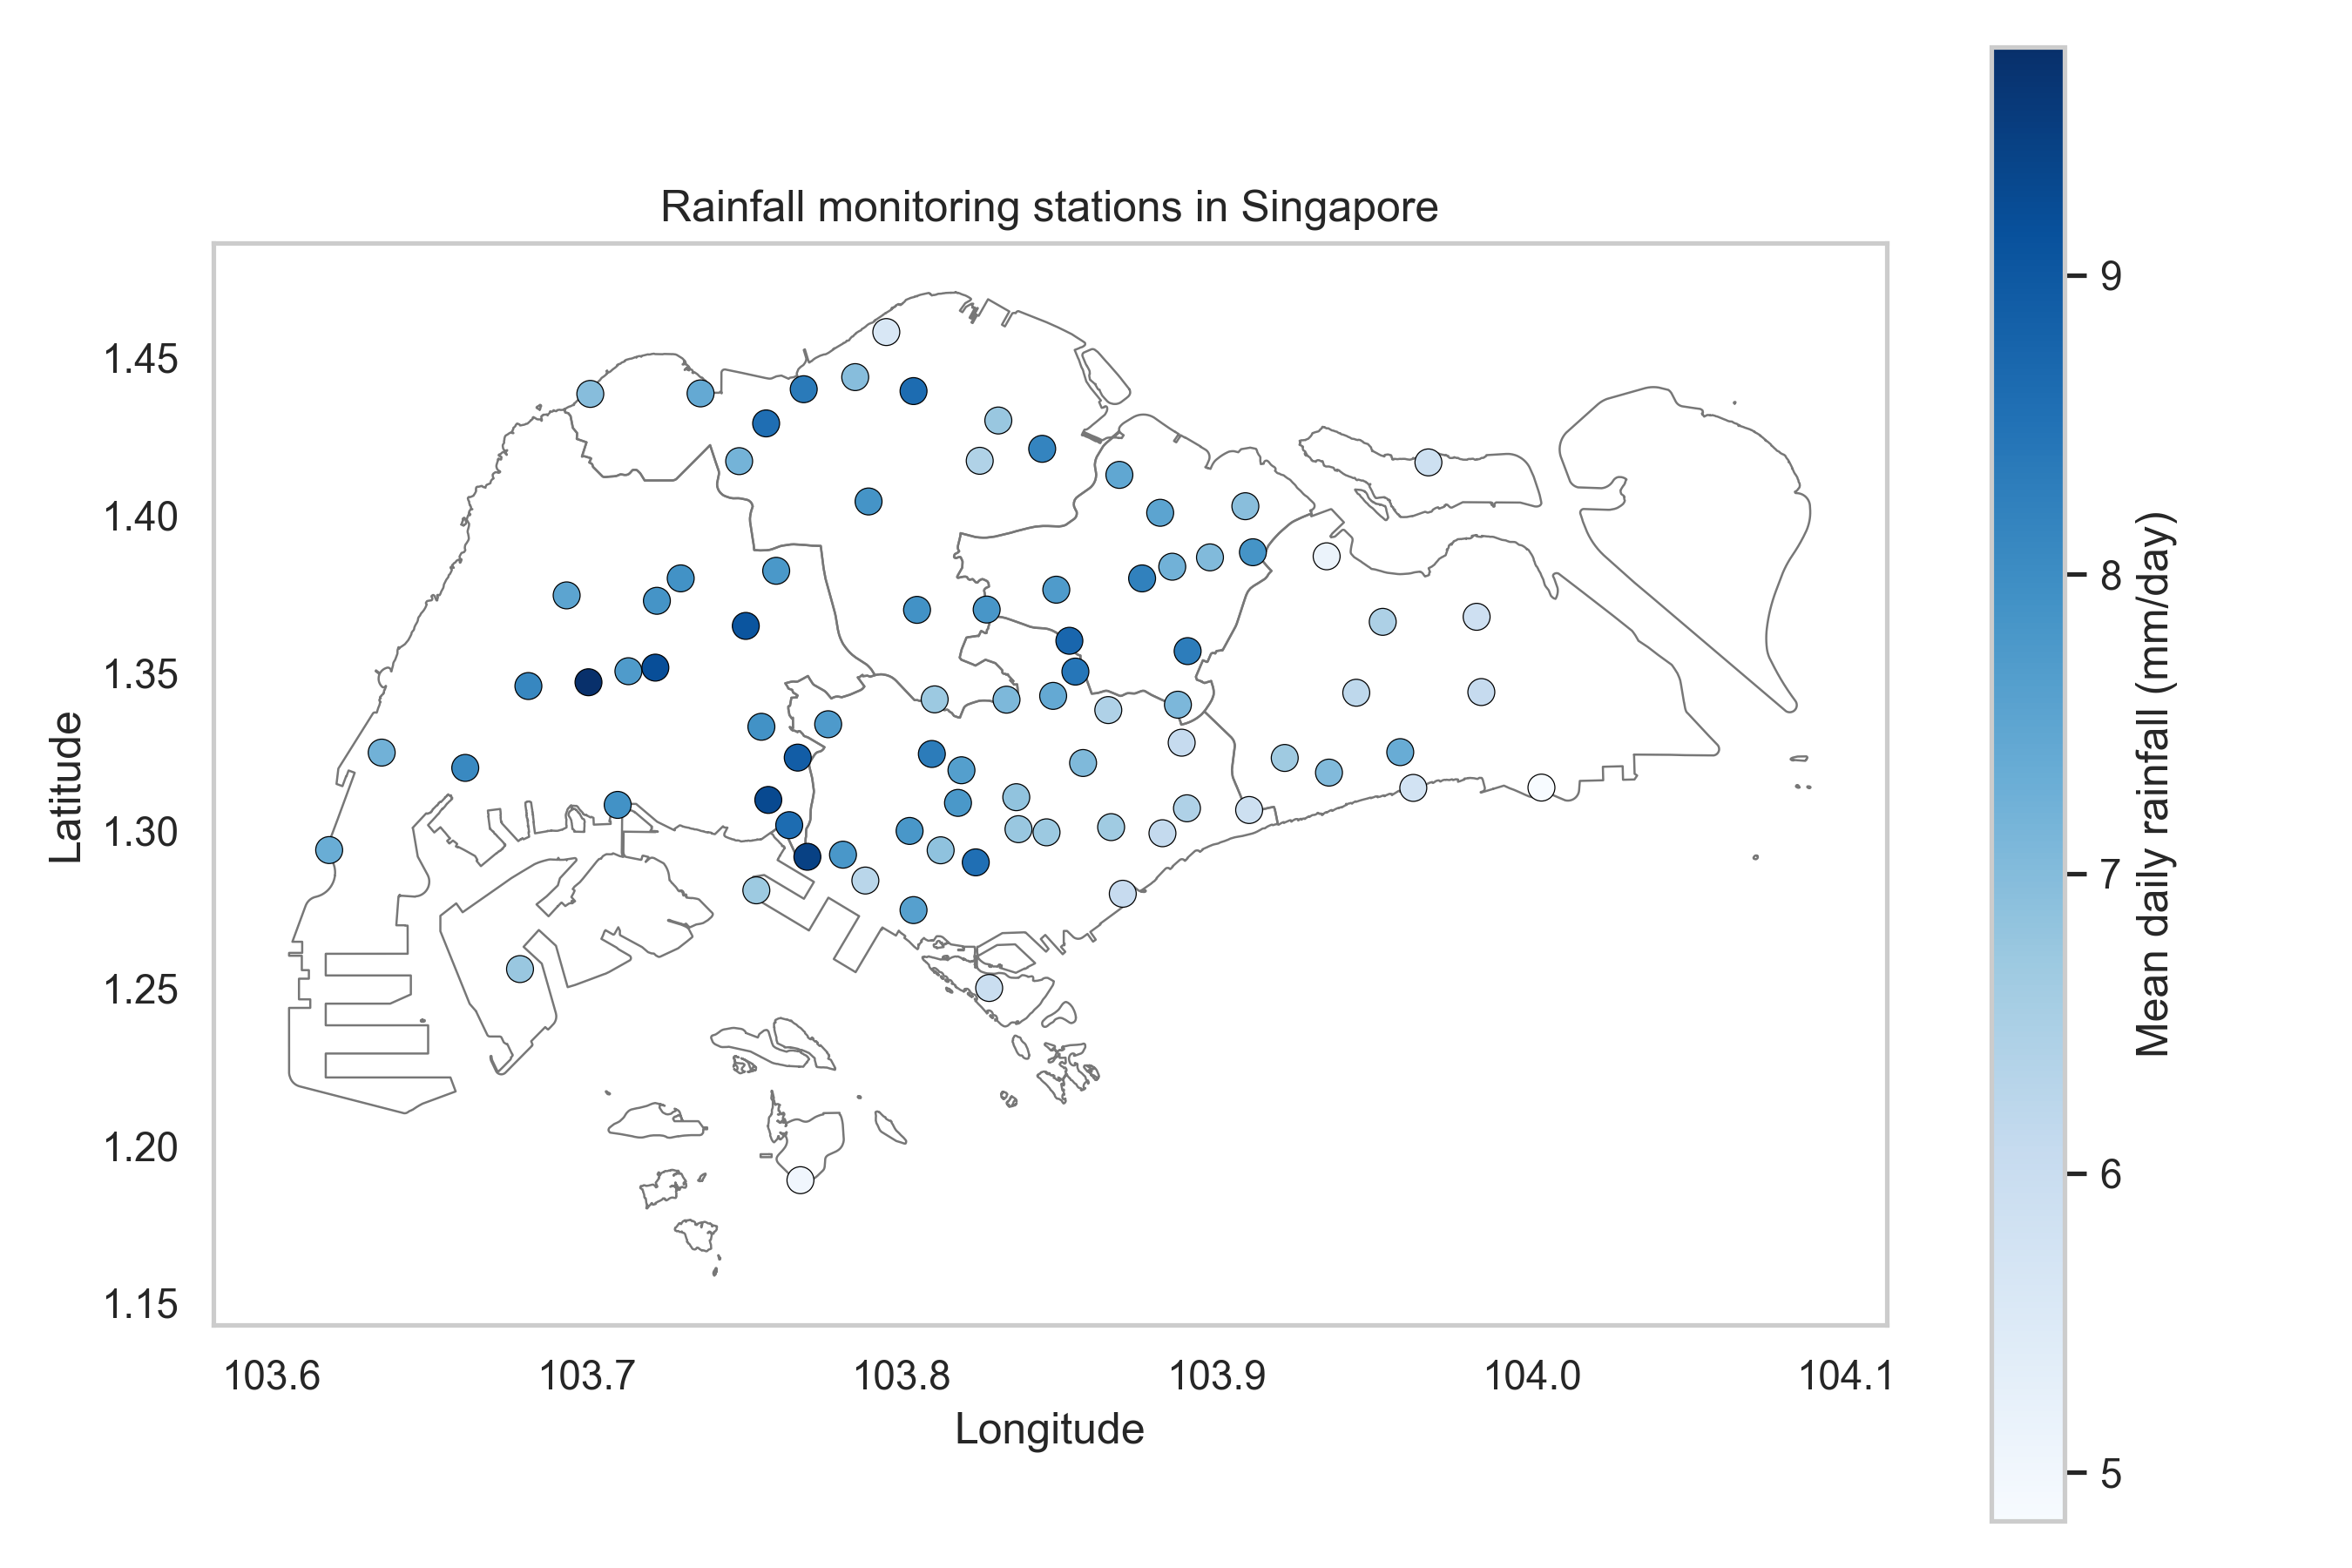
\includegraphics[width=0.9\textwidth]{figures/station_map.png}
    \caption{Mean daily rainfall at monitoring stations with at least 365 valid
    days.}
    \label{fig:stations}
\end{figure}

\subsection{Summary of findings}

In summary, rainfall varied noticeably between years, months, hours, and
stations. The wettest year in the analysed period was 2022 and the driest was
2019. November had the highest average rainfall across the eight years, while
the afternoon, especially around 15:00, had the clearest hourly peak. The
station map also showed meaningful differences between locations. These
results suggest that year, month, hour, and station information are all useful
when describing rainfall and when selecting features for the prediction task.

\end{document}
